\section{Discussion}
\noindent \textbf{Needle‑in‑a‑Haystack.}
\begin{figure}[t]
  \centering
  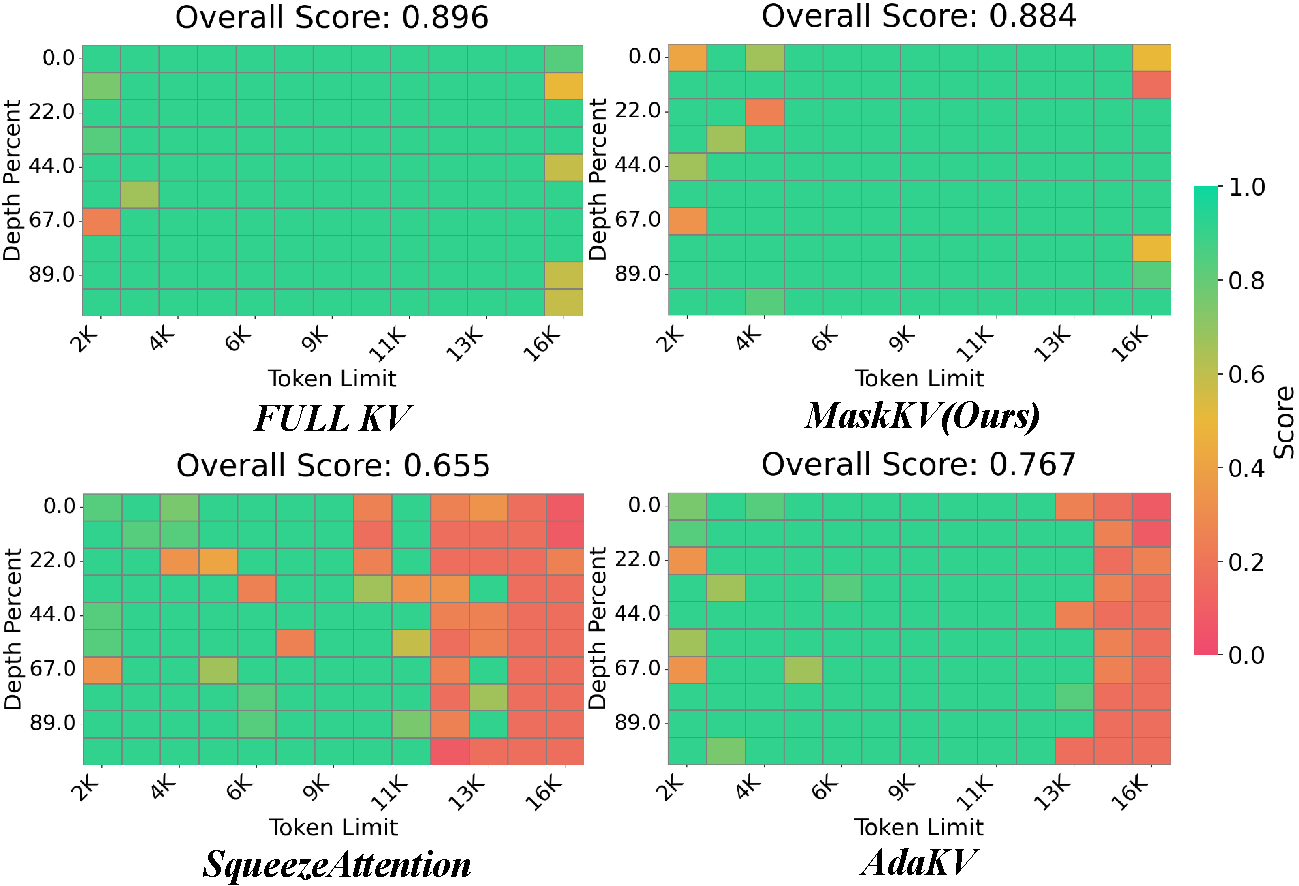
\includegraphics[width=\columnwidth]{figure/NIAH_LLADA.pdf}
    \caption{A visualization from the Needle-in-a-Haystack test. See Figure~\ref{fig:niah_all} for full results.}
  \label{fig:needle}
\end{figure}
To better understand the model’s ability to retrieve fine‑grained information hidden within long contexts, we conduct a preliminary study using the “needle‑in‑a‑haystack” setup (see Fig.~\ref{fig:needle}). Our method shows stronger robustness to increasing prompt length, effectively maintaining information retrieval performance.

\noindent \textbf{Visualization of Prompt Preference.}

As shown in Fig.~\ref{fig:prefer}, we analyze the prompt preference distribution across different heads within the same layer. Some heads allocate substantial attention to the prompt, likely to extract task-relevant information, while others focus more on the masked region to plan answer generation. Such analysis provides deeper insight into their internal decision behavior.

\begin{figure}[H]
  \centering
  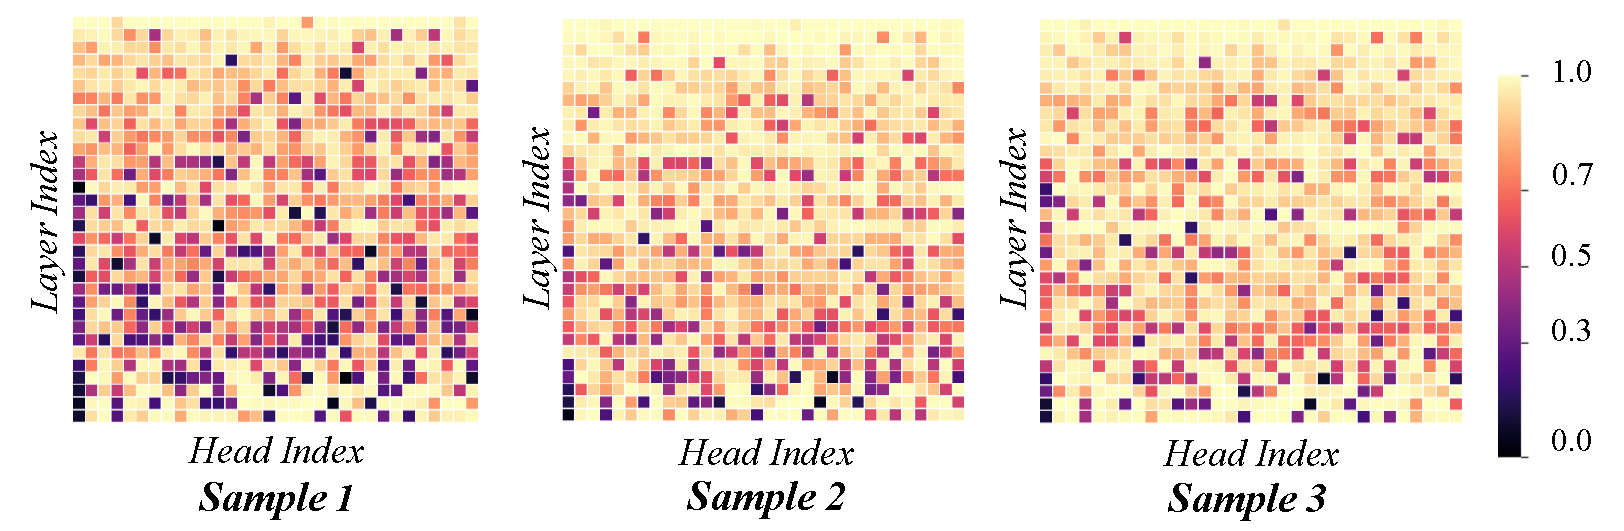
\includegraphics[width=\columnwidth]{figure/prefer.pdf}
  \caption{Visualization of Prompt Preference.}
  \label{fig:prefer}
\end{figure}

\noindent \textbf{ Comparison of Voting Strategies.}
We analyze voting strategies by grouping masked tokens into front, middle, and back regions, each contributing a position-specific vote. Results (Tab.~\ref{tab:mask_voting_position}) show that later positions yield more accurate votes for identifying critical tokens, suggesting position-aware voting may further improve eviction effectiveness.


